\documentclass{article}
\usepackage[utf8]{inputenc}
\usepackage{geometry}
\usepackage{tikz}
\usepackage{amsmath}
\usepackage{listings}
\usepackage{xcolor}
\usepackage{graphicx}
\graphicspath{ {./images/} }

\geometry{
 a4paper,
 total={170mm,257mm},
 left=20mm,
 top=20mm,
 }
\setlength{\parindent}{0pt}
\setlength{\parskip}{0.8em}

\title{CMT316: Coursework 2 - Computer Vision}
\author{CV4 Group}
\date{1 June 2021}

\begin{document}

\maketitle

\section{Introduction}

Explain the task
Assume the reader understands ML and CV, but doesn't know this task


\section{Dataset Overview}

The VOC2012 combined training and validation data sets contain 11,540 images and their associated annotations. For the purposes of our project, we have used the training and validation sets provided by VOC2012 as the full data set and made our own partition of the data as discussed below in the Methodology. The images all contain at least one object that is identified as one of 20 classes. Images may contain more than one identified object. 

The images are provided as jpeg files. The annotations are provided in XML format. Each annotation contains information about the size of the image (height, width, number of channels), as well as the class and bounding box of each identified object within the image. The bounding boxes of the objects are defined by the coordinates of the four corners of the box (xmin, xmax, ymin, ymax). Listing \ref{lst:label} gives an example of the format of the annotation information.

\begin{lstlisting}[language=XML, label={lst:label}, caption=Annotation example]
<annotation>
	<folder>VOC2012</folder>
	<filename>2007_000027.jpg</filename>
	<source>
		<database>The VOC2007 Database</database>
		<annotation>PASCAL VOC2007</annotation>
		<image>flickr</image>
	</source>
	<size>
		<width>486</width>
		<height>500</height>
		<depth>3</depth>
	</size>
	<segmented>0</segmented>
	<object>
		<name>person</name>
		<pose>Unspecified</pose>
		<truncated>0</truncated>
		<difficult>0</difficult>
		<bndbox>
			<xmin>174</xmin>
			<ymin>101</ymin>
			<xmax>349</xmax>
			<ymax>351</ymax>
		</bndbox>
	</object>
</annotation>

\end{lstlisting}


\textbf{Distribution of objects across the classes:}

Taking the label of the first object listed in the annotation file for each image as the 'primary object' of the image, the distribution of these primary objects is not across the classes. Figure \ref{fig:image_by_class} shows that 'person' is the most common primary object for an image, followed by 'dog' and 'cat'; 'dining table' is the least frequent primary object. As a \% of total images, their relative frequency ranges from 16.9\% for 'person' to 2.0\% for 'dining table. The full breakdown of the primary object by class for the training, validation and development sets is given in Figure \ref{fig:data_overview} in the Appendix.

\begin{figure}[h]
  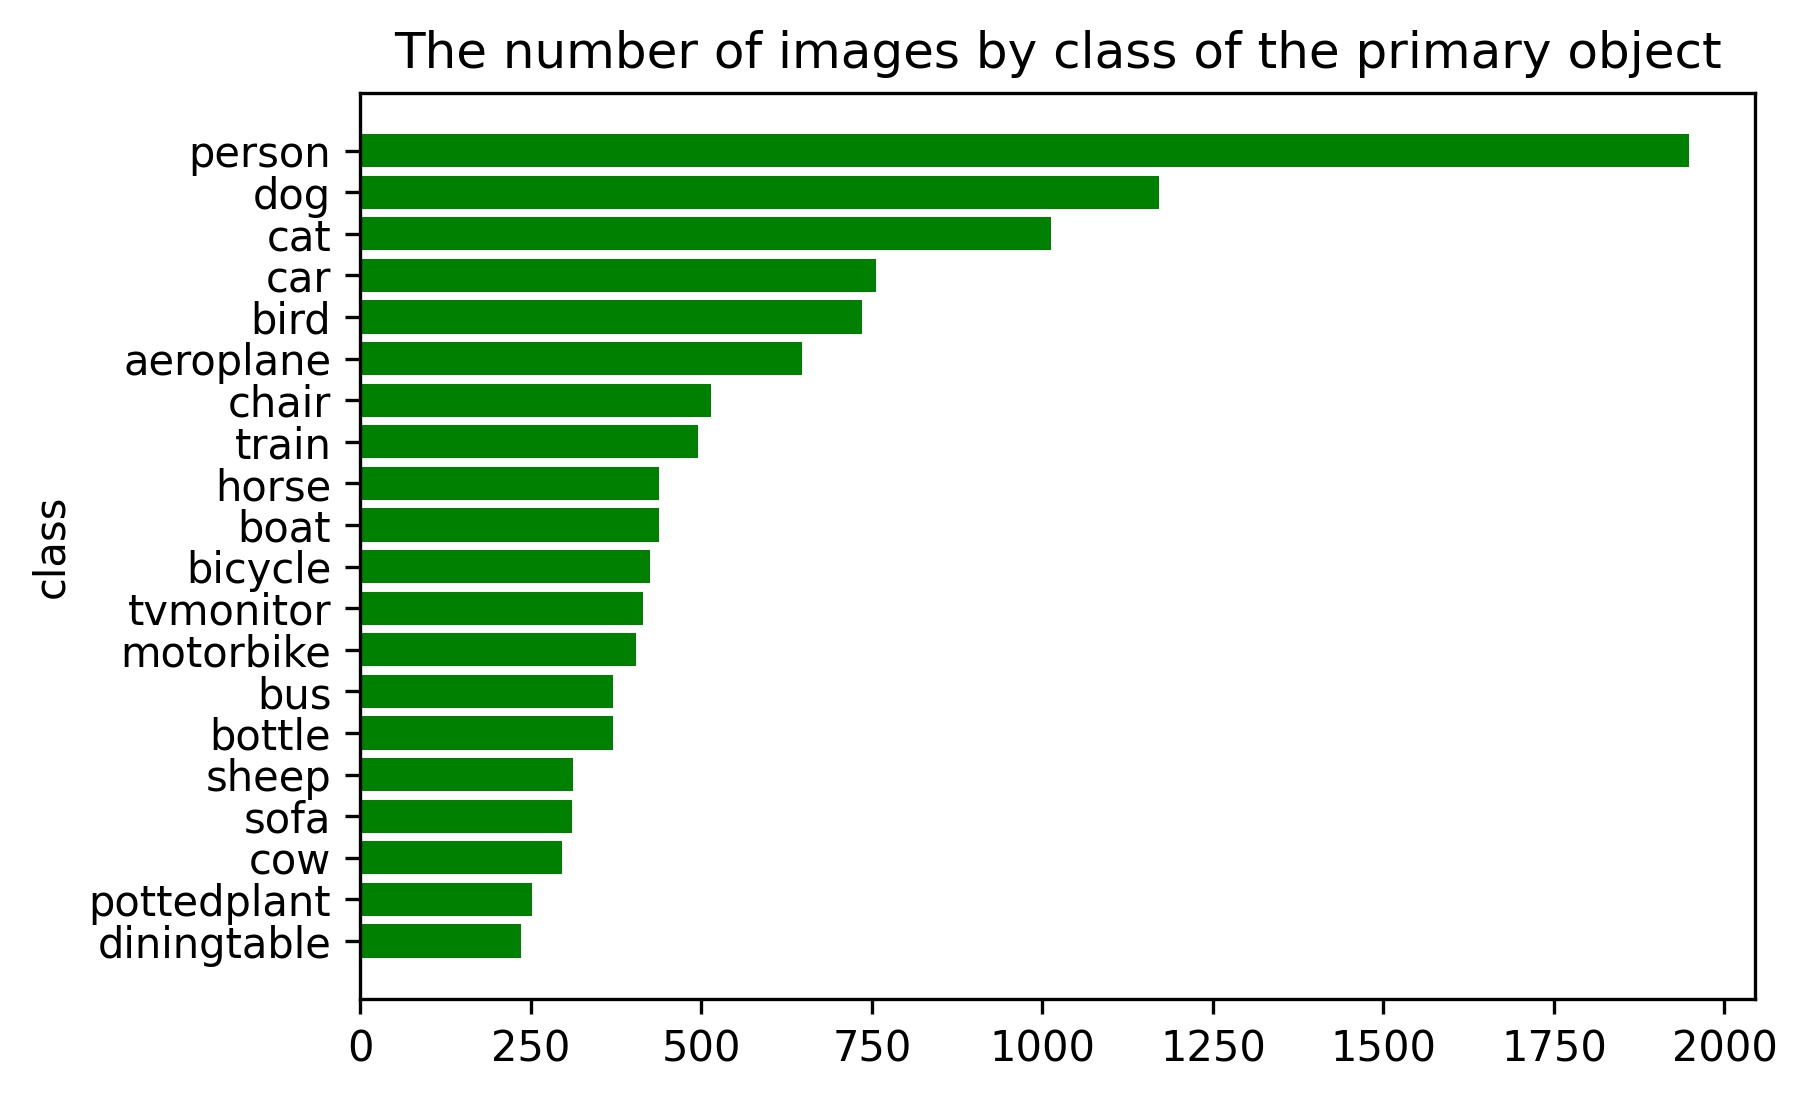
\includegraphics[scale = 0.7]{bar_channels.jpg}
  \centering
  \caption{Distribution of Images by Primary Object Class}
  \label{fig:image_by_class}
\end{figure}


\textbf{The number of objects in each image:}

The images in the data set contain a variable number of located objects per image. The most common number of objects in an image is 1. However, 52\% of images have 2 or more objects identified and the maximum number of objects identified in an image is 39. Figure \ref{fig:objects_by_image} summarises the distribution of the number of objects per image in the data set:

\begin{figure}[h]
  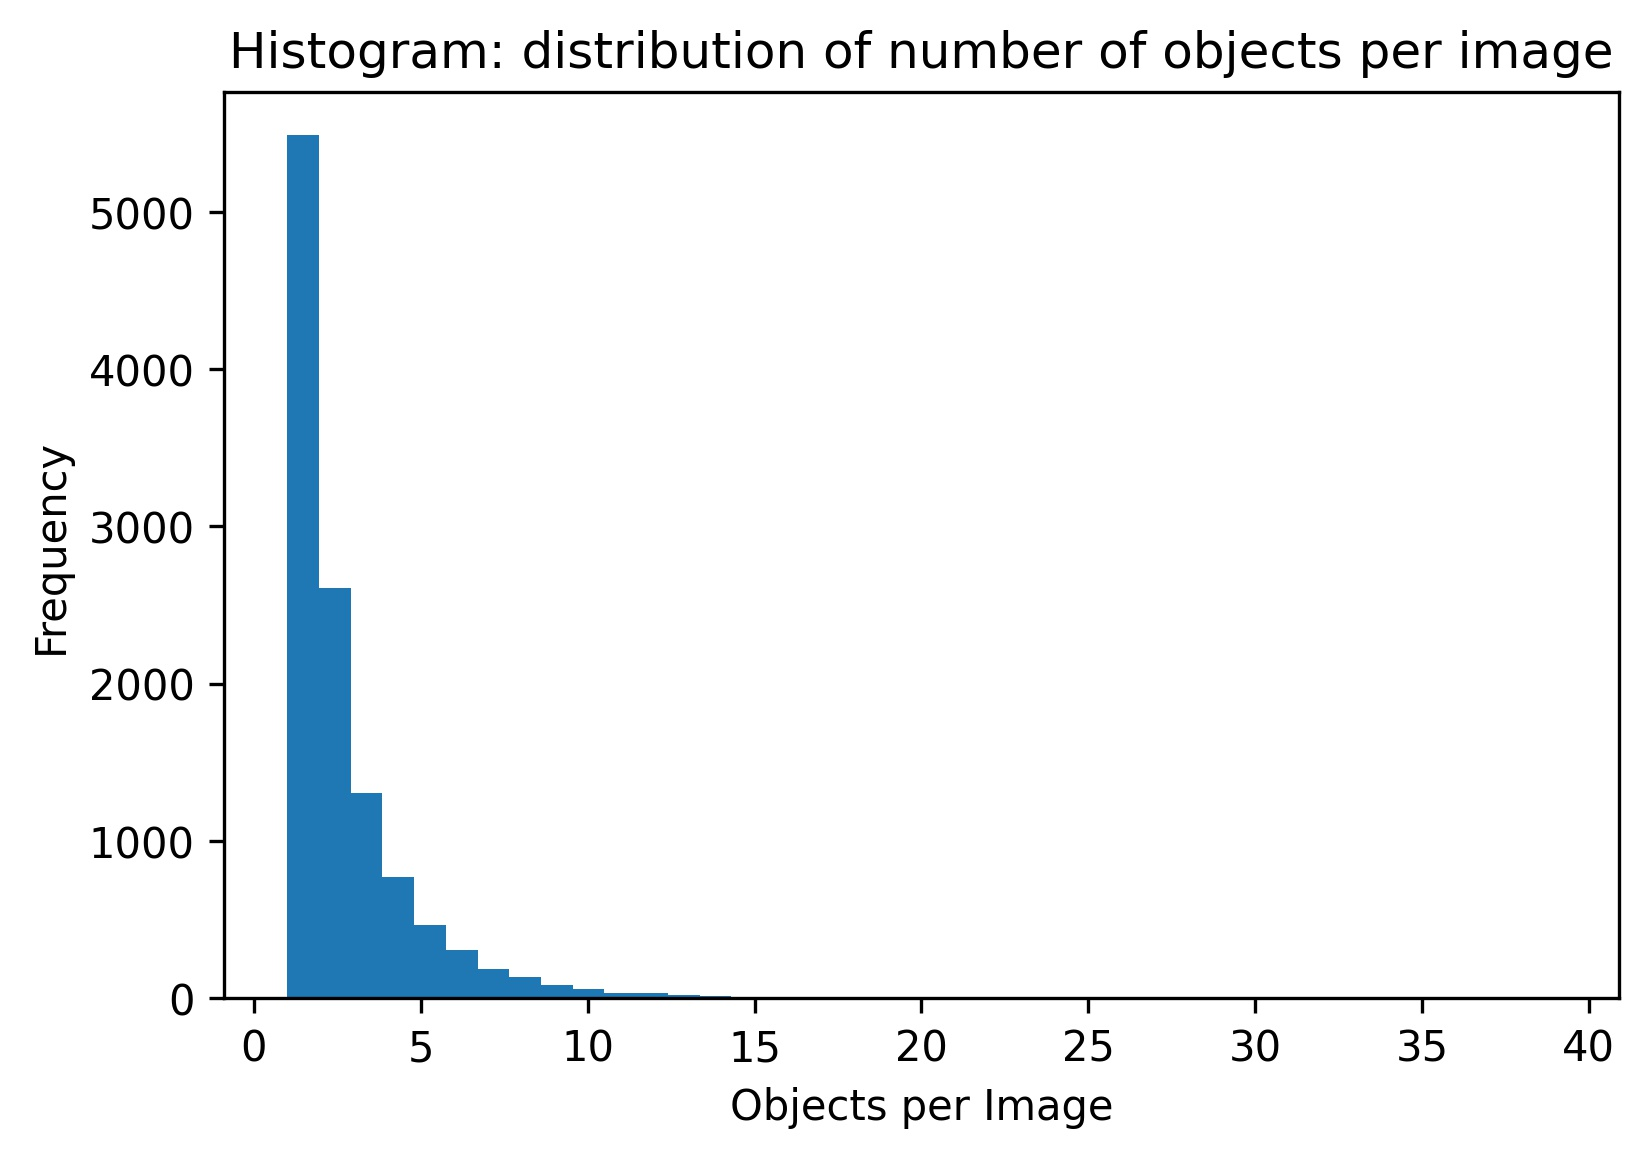
\includegraphics[scale = 0.7]{hist_objects.jpg}
  \centering
  \caption{Distribution of Number of Objects per Image}
  \label{fig:objects_by_image}
\end{figure}


\textbf{Image sizes:}

The images are different sizes and aspect ratios: 772 unique image sizes occur in the data set. Typically a pre-trained model will expect images to be resized to a specific size as input to the model (For example, the resnet50 model expects images of size 224 x 224). Image resizing functions such as \lstinline{img_load_img} in keras do not maintain the aspect ratio of the original image, it is 'squished' down to size. This is noted as a potential factor in the relative performance of the model on some images vs. others. Figure \ref{fig:objects_by_image} shows the frequency of the top 10 most frequent image sizes. Approximately 40\% of the images are 500 x 375 but there is a long tail of image sizes.

\begin{figure}[h]
  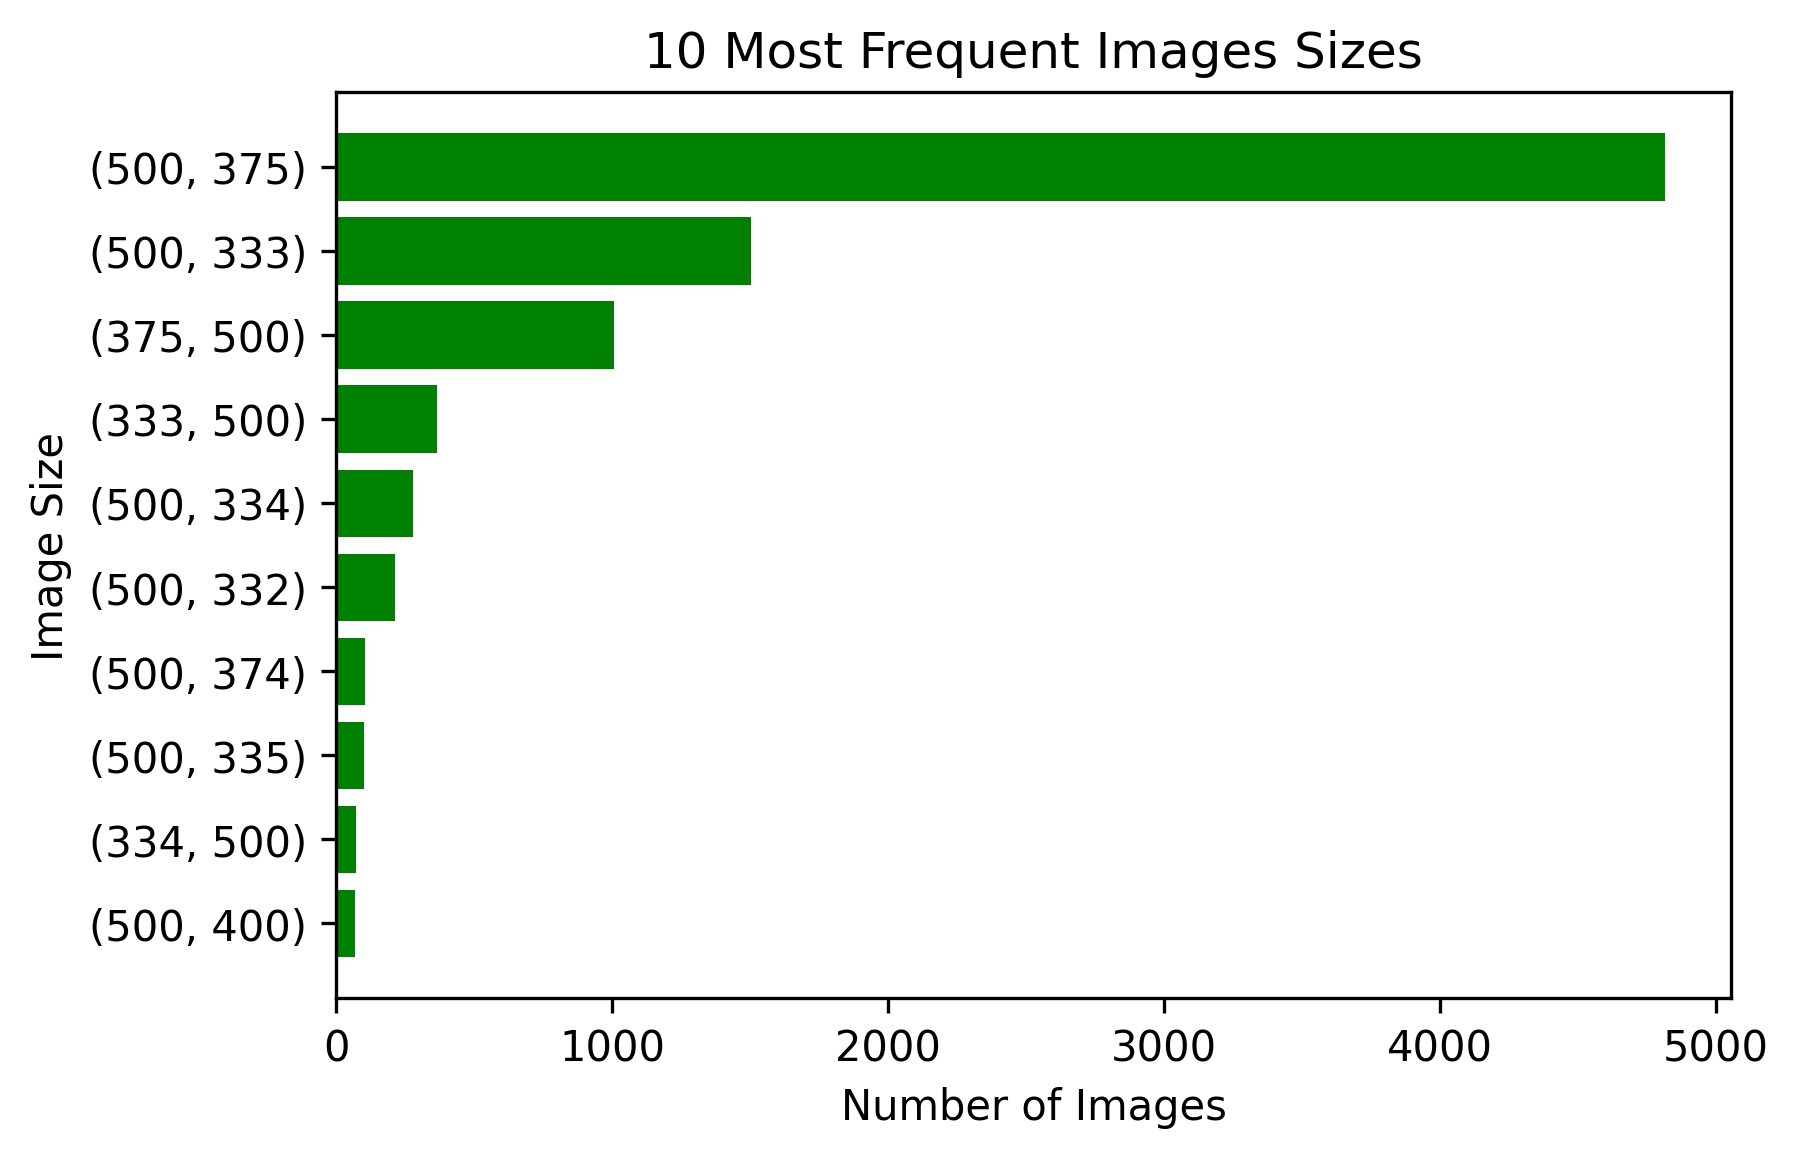
\includegraphics[scale = 0.7]{aspect_ratio.jpg}
  \centering
  \caption{Top 10 most Frequent Image Sizes}
  \label{fig:aspect_ratios}
\end{figure}

\textbf{Bounding boxes:}

The bounding box provided for each object describes the coordinate of four corners of a rectangle that surrounds the object. An annotated image contains a bounding box drawn around each identified object, and the label of the class of that object associated with the box. Figure \ref{fig:bounding_boxes} illustrates that the bounding boxes may overlap.

\begin{figure}[h]
  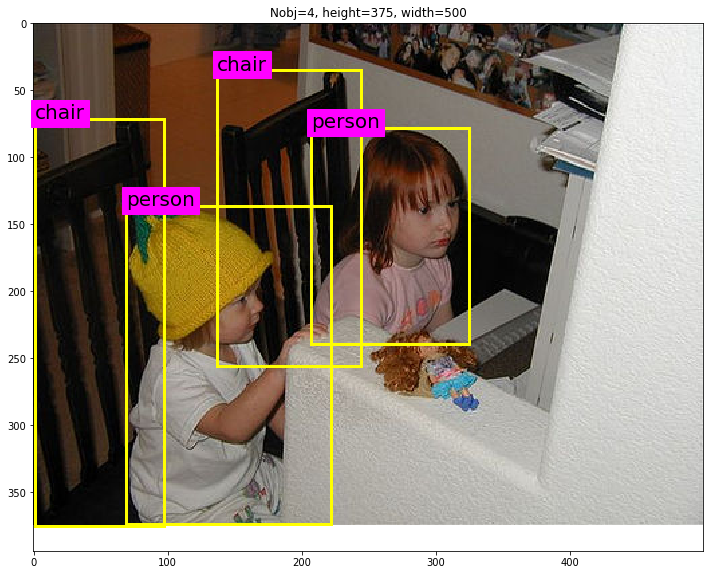
\includegraphics[scale = 0.3]{bbox_example.png}
  \centering
  \caption{An Example of an Annotated Image}
  \label{fig:bounding_boxes}
\end{figure}


\section{Methodology}

Discussion of the pre-processing steps:
- explain the encoding of the images for the different models
- Explain transformation of xml to txt files, and compilation of dataframe for label data - the pre-processing steps that were valuable to all of the models.

Discussion of some of the issues in pre-processing the data:
- explain run time and timeout issues and experiments to share pre-processed images by csv, npy files etc.
- Explain that we initially tried to convert the images to csv, .npy in order to pre-process once and share the raw data. We should have looked at the model inputs more closely before attempting that process as the implementations of the Faster R-CNN and Yolo v3 models are different some of the pre-processing is built into the model. Some of the pre-processing steps were unncessary.

Discussion of the models used in the project, in particular Faster R-CNN and Yolo v3.

\section{Experimental Setting}

Description of the specific details of the evaluation - e.g. parameter tuning, use of the development set


\section{Results}

Final results of the experiments, including baselines, tables metrics (IoU and classification metrics)

For the classification
- accuracy
- precision
- recall
- macro-f1

For the object localisation:
- intersection over union - IOU

\section{Analysis}

Discussion of the results
Include error analysis - go into the data, pull out the specific examples and explain why the model is working or not working. Look at the predictions for each instance, based on the errors that the model is making, try to improve the model and fix the errors.

[ADVICE FROM JOSE - Include failed attempts - they are valid attempts. Will be rewarded for sensible ideas, if all sounds good and correctly implemented, and then critically evaluated. Don't expect 100\% performance, but explain why the performance is low, e.g. in terms of the network architecture - too simple so underfit].

[NOTE - THIS IS WHERE WE NEED TO INCLUDE THE DISCUSSION OF SHAOSHI'S FAILED ATTEMPTS TO TRAIN THE YOLO V3 MODEL IN KERAS, BEFORE MOVING TO TORCH]


\section{Literature Review}

What models work well?
What is the standard that is used
Link the research to what we have done - explain why we chose what we did - e.g.
some models may require more compute power than we have


\section{Conclusion and Future Work}

Discussion of ways to improve the work in the future:

- example (if relevant to the Faster R-CNN and Yolo) - rather than using default resizig, rescaling along the longest size and maintaining the aspect radio and padding the remainder of the image may be a better approach to improve performance in the models.

\section{Appendix}
\begin{figure}[h]
  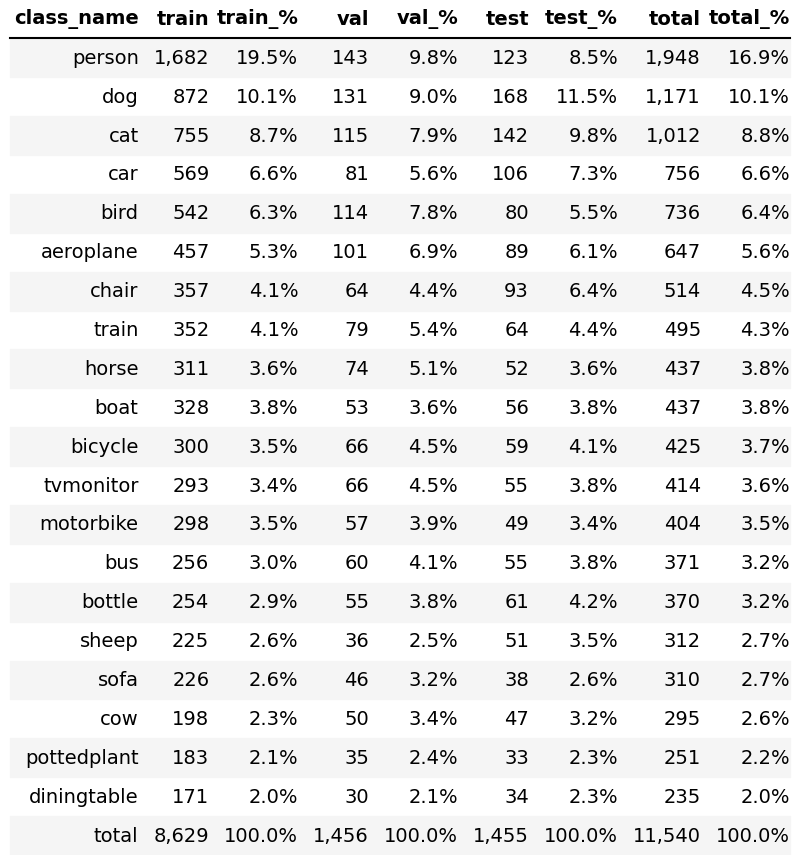
\includegraphics[scale = 0.5]{df_styled.jpg}
  \centering
  \caption{Distribution of Images by train, val, test by Class}
  \label{fig:data_overview}
\end{figure}

\end{document}
